\documentclass[11pt,letterpaper]{article}
\usepackage{acl2013}
\usepackage[lowtilde]{url}
%\usepackage[colorlinks]{hyperref}  % messes up our bib format, and doesn't work with Author (Year) citations
\usepackage{times}
\usepackage{latexsym}
\usepackage{amsmath}
\usepackage{amssymb}
\usepackage{amsthm}
\usepackage{enumerate,paralist,enumitem}
\usepackage{verbatim}
\usepackage{mathtools}

\usepackage{array}

\usepackage{graphicx}
\usepackage{caption,subcaption}
\usepackage{algorithm}
\usepackage{algorithmic}

\DeclareMathOperator*{\argmax}{arg\,max}

%\usepackage{authordate1-4}
\usepackage{multirow}

\usepackage{color,soul}
\usepackage{transparent}
\usepackage[usenames,dvipsnames,svgnames,table]{xcolor}
\newcommand{\Note}[1]{}
\renewcommand{\Note}[1]{\hl{[#1]}}  % comment this out to remove notes
\newcommand{\FIXME}{\Note{FIXME}}
\newcommand{\NoteSigned}[3]{{\sethlcolor{#2}\Note{#1: #3}}}
\newcommand{\RemoveFF}[1]{\NoteSigned{Remove (FF)}{Crimson}{#1}}
\newcommand{\NoteFF}[1]{\NoteSigned{FF}{LightBlue}{#1}}
\newcommand{\NoteJE}[1]{\NoteSigned{JE}{LightGreen}{#1}}
\newcommand{\Commented}[1]{#1}

\newcommand{\empirical}[0]{\ensuremath{\tilde{p}}}
\newcommand{\Data}[0]{\ensuremath{\mathcal{D}}}

\newcommand{\WhereToFind}[0]{\url{http://cs.jhu.edu/~jason/tutorials/loglin/}}

%%%%%%%%%%%%%%%%%5
%CHANGE THIS!!!
\newcommand{\NumLessons}[0]{18}% \NoteFF{change \#: 18}}

\setlength\titlebox{6.5cm}    % Expanding the titlebox


\title{A Virtual Manipulative for Learning Log-Linear Models}


\author{
Francis Ferraro \and Jason Eisner\\
Department of Computer Science\\
Johns Hopkins University\\
Baltimore, MD, USA
}
  
\date{}

\begin{document}

\maketitle

\begin{abstract}
  We present an open-source virtual manipulative for conditional
  log-linear models. This web-based interactive visualization lets
  the user tune the probabilities of various shapes---which grow and
  shrink accordingly---by dragging sliders that correspond to feature
  weights.  The visualization displays a regularized training
  objective; it supports gradient ascent by optionally displaying
  gradients on the sliders and providing ``step'' and ``solve''
  buttons.  The user can sample parameters and datasets of
  different sizes and compare their own parameters to the truth.  Our
  website, \WhereToFind{}, guides the user through a series of
  interactive lessons.%
  % and also provides a handout with a more formal
  % treatment.
  \NoteJE{mention associated homework exercises if we are
    definitely going to provide them}
  % Included with our system are auxiliary instructional
  % materials and questions usable for assignments. 
\end{abstract}

\section{Introduction}\label{sec:intro}
We argue that if one is going to teach only a single machine learning
technique in a computational linguistics course, it should be {\em
  conditional log-linear modeling}.  Such models are pervasive in
natural language processing.  They have the form
\begin{equation}\label{eqn:loglin}
p_{\vec{\theta}}(y \mid x) \propto \exp{\left(\vec{\theta} \cdot \vec{f}\left(x,y\right)\right)},
\end{equation}
where $\vec{f}$ extracts a feature vector from context $x$ and
outcome $y \in \mathcal{Y}(x)$.  The set of possible
outcomes $\mathcal{Y}(x)$ might depend on the context
$x$.\footnote{The model is equivalent to logistic regression
  when $y$ is a binary variable, that is, when $\mathcal{Y}(x)=\{0,1\}$.}

We then present an interactive web visualization that guides students
through playing with log-linear models and their estimation. This open-source 
tool, available at \WhereToFind{}, is intended to develop intuitions, so that basic
log-linear models can be then taken for granted in future lectures.  It can be used near
the start of a course, perhaps after introducing probability notation
and $n$-gram models.

\begin{figure*}
\centering
%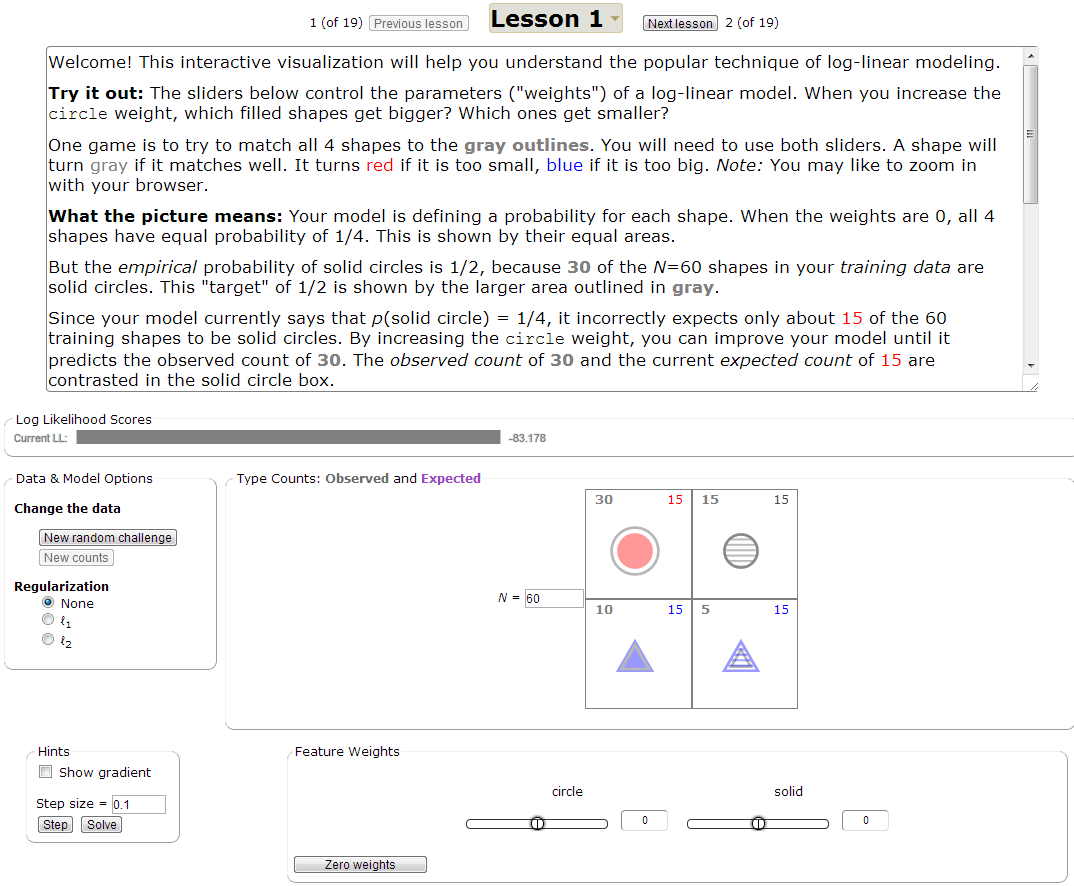
\includegraphics[scale=.49]{images/lesson1-051313-intro-zoom-instmore.PNG}
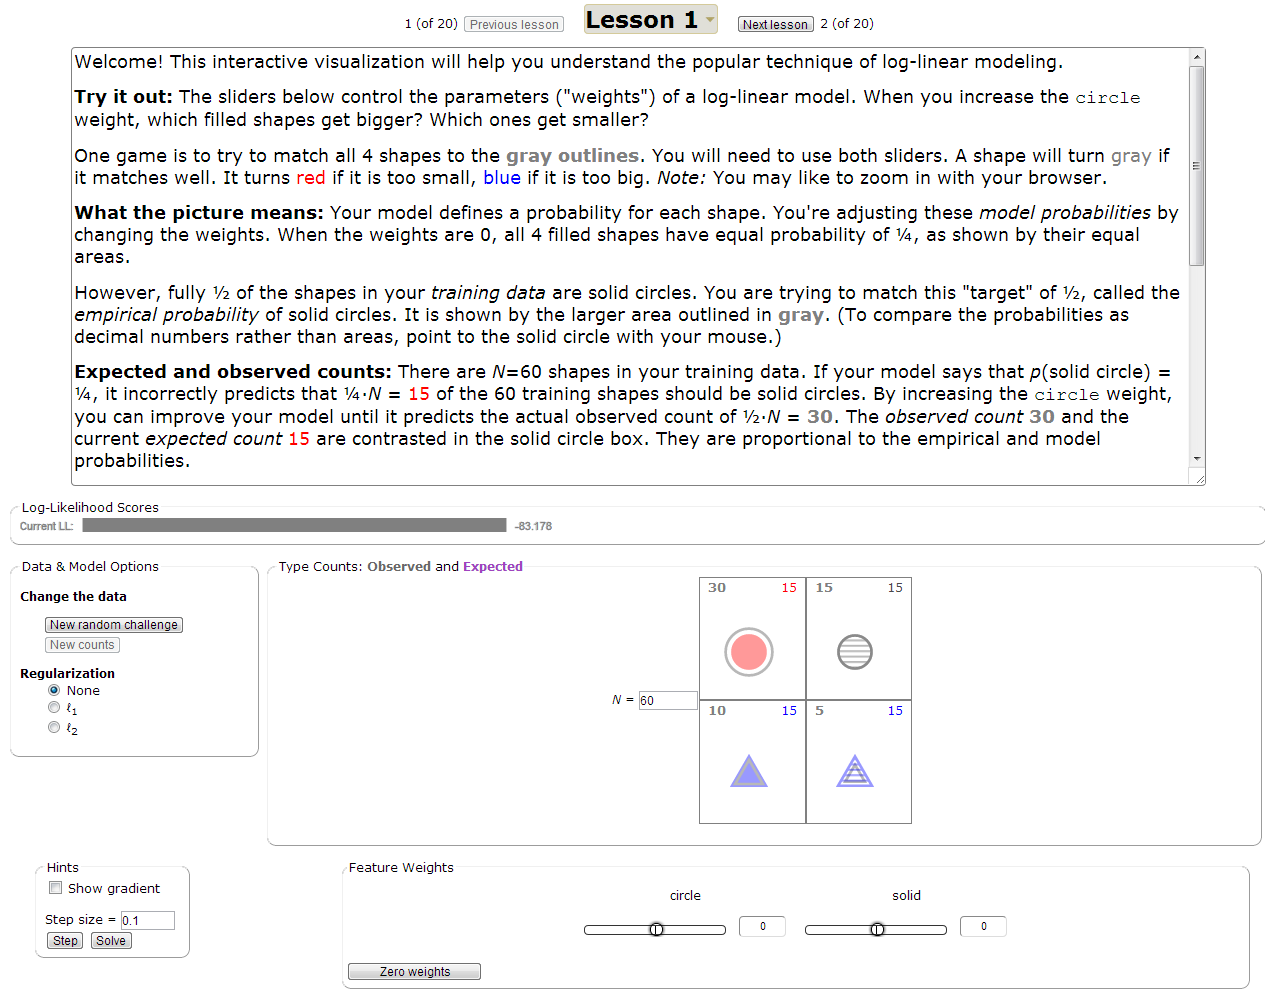
\includegraphics[scale=.435]{images/lesson1-060713-intro-zoom-3.PNG}
\caption{The first lesson; the lower half is larger on the actual
  application.}
\label{fig:lesson1}
\end{figure*}

We used the tool in our Natural Language Processing (NLP) class and received
very positive feedback.  Students were excited by it, with some saying
the tool helped develop their ``physical intuition'' for log-linear
models.
%\NoteJE{they did? who?}  
%\NoteFF{Students, either through email, comments in homework assignments 
%or one-on-one discussions. I can send names via email if you like.}
Other test users with no 
% statistical, computational, or
technical background also enjoyed working
through the introductory lessons and found that they began to understand 
the model.

The app includes \NumLessons{} ready-to-use lessons for individual or
small-group study or classroom use.  Each lesson, e.g. Figure
\ref{fig:lesson1}, guides the student to fit a probability model $p_{\vec{\theta}}(y \mid
x)$ over some collection ${\cal Y}$ of shapes, words, or other images
such as parse trees.  Each lesson is peppered with questions; students
can be asked to answer some of these questions in
writing.\footnote{There are approximately 6 questions per lesson. We
  found that answering {\em all} the questions took our students about
  2300 words, or just under 23 words per question, which was probably
  both unreasonable and unnecessary.}  Ambitious instructors can add new
lessons or edit existing ones by writing configuration files (see
section~\ref{sec:tailoring}). This is useful for emphasizing specific
concepts or applications.
% ; instructors may also use it to prepare students for any upcoming assignments.  
Section \ref{sec:history} provides some history and applications of log-linear
modeling, as well as assignment ideas.

\section{Why Teach With Log-Linear Models?}

Log-linear models are very handy in NLP.  They can be used {\em throughout} 
a course, when one needs 
\begin{itemize}
\item a global classifier for an applied task, such as detecting
  sentiment, topic, spam, or gender;
\item a local classifier for structure annotation,
  such as tags or segment boundaries;
\item a local classifier to be applied repeatedly in sequential decision-making;
\item a local conditional probability within some generative process, such
  as an $n$-gram model, HMM, PCFG, probabilistic FSA or FST, noisy-channel MT model,
  or Bayes net;
\item a global structured prediction method.  Here $y$ is a complete
  structured object such as a tagging, segmentation, parse, alignment, or translation.  Then $p(y
  \mid x)$ is a Markov random field or a conditional random field,
  depending on whether $x$ is empty or not.
\end{itemize}  

Log-linear models over discrete variables are also sufficiently
expressive for an NLP course.  Students may experiment freely with
adding their own creative model \textit{features} that refer to 
salient \textit{attributes} or \textit{properties} of the data, 
since the probability \eqref{eqn:loglin} may consider any number of
informative features of the $(x,y)$ pair.

How about training?  Estimation of the parameter weights
$\vec{\theta}$ from a set of fully observed $(x,y)$ pairs is simply a
convex optimization problem.  Maximizing the regularized maximum
likelihood
\begin{equation}\label{eqn:reg_ll}
% \argmax_{\vec{\theta}} \sum_i \log p_{\vec{\theta}}(y_i \mid x_i) - C\cdot R\left(\vec{\theta}\right)
  F(\vec{\theta}) = \sum_{i=1}^N \log{p_{\vec{\theta}}\left(y_i\ \mid\ x_i\right)} - C \cdot R(\vec{\theta})
\end{equation}
is a simple, uniform training principle that can be used throughout
the course.  The scaled regularizer $C\cdot R(\vec{\theta})$
prevents overfitting on sparse features.
This is arguably more straightforward than the traditional NLP
smoothing methods for estimating probabilities from sparse data
\cite{chen-goodman-1996}, which require applying various {\em ad hoc}
formulas to counts, and which do not generalize well to settings where
there is not a natural sequence of backoff models.  There exist 
fast and usable tools that students can use to train their log-linear
models, including, among others, MegaM \cite{daume04cg-bfgs}, 
and NLTK \cite{bird2009natural}.\footnote{\label{fn:bigY}A caveat is that generic
  log-linear training tools will {\em iterate} over the set ${\cal
    Y}(x)$ in order to maximize
  \eqref{eqn:loglin} and to compute the constant of proportionality
  in \eqref{eqn:loglin} and the gradient of
  \eqref{eqn:reg_ll}.  This is impractical when ${\cal Y}(x)$ is large, as in
  language modeling or structured prediction.  See Section \ref{sec:history}.
%One will do better to
% either restrict ${\cal Y}(x)$ before training
%\cite{johnson-et-al-1999}, or else use techniques such as dynamic
%programming or sampling, e.g., 
%\cite{lafferty-mccallum-pereira-2001} and \cite{rosenfeld-chen-zhu-2001}. 
%These often exploit special
%structure in the feature set; students will have to use other tools or 
%write their own code.\label{fn:compute_partition_fn}
}

Formally, log-linear models are a good gateway to a more general
understanding of undirected graphical models and the exponential
family, including globally normalized joint or conditional
distributions over trees and sequences.

One reason that log-linear models are both versatile and pedagogically
useful is that they do not just make predictions, but explicitly 
model {\em probabilities}.  These can be 
\begin{itemize}
\item combined with other probabilities using the usual rules of probability;
\item marginalized at test time to obtain the probability that the outcome 
  $y$ has a particular property (e.g., one can sum over alignments);
\item marginalized at training time in the case of incomplete data $y$
  (e.g., the training data may not include alignments);
\item used to choose among possible decisions by computing their 
  expected loss (risk).
\end{itemize}
The training procedure also takes a probabilistic view.  Equation
\eqref{eqn:reg_ll} helps illustrate important statistical principles such as maximum
likelihood, regularization (the bias-variance tradeoff), and cross-validation, as well as
optimization principles such as gradient ascent.\footnote{In an
  advanced class, this objective can also be regarded as the
  optimization dual of a maximum entropy problem.  We have considered
  adding a dual view to our manipulative.\label{fn:dual}}

Log-linear models also provide natural extensions of commonly taught
NLP methods.  For example, under a probabilistic context-free
grammar (PCFG),\footnote{Likewise for Markov or hidden Markov models.}  $p(\text{parse tree}\mid\text{sentence})$ is proportional to
a product of rule {\em probabilities}.  Simply replacing each rule
probability with an arbitrary non-negative {\em potential}---an
exponentiated weight, or sum of weights of features of that
rule---gives an instance of \eqref{eqn:loglin}.  The same parsing
algorithms still apply without modification, as does the same
inside-outside approach to computing the posterior expectation of rule counts and 
feature counts.  Immediate variants include CRF CFGs
\cite{finkel2008efficient}, in which the rule features become
position-dependent and sentence-dependent, and log-linear PCFGs
\cite{bergkirkpatrick-et-al-2010}, in which the feature-rich rule
potentials are locally renormalized into rule probabilities via
\eqref{eqn:loglin}.

% OLD VERSION
% Further, underlying concepts of log-linear models may tie in nicely with known 
% NLP algorithms. For instance, log-linear models can help teach weighted grammars and 
% sequence models. Consider either ordinary probabilistic CKY (HMMs). The joint probabilities 
% over a sentence and some proposed \texttt{structure} are simply products of individual probabilities 
% (which of course could themselves be modeled by conditional log-linear distributions); 
% normalizing results in $p(\texttt{structure} | \textrm{sentence})$. 
% Next, using properties of logarithms and exponents we can replace the \textit{log probabilities} 
% in the above conditional distribution with arbitrary weights or sums of weights. We can still use the well-known
% inside-outside (forward-backward) algorithms, but now use non-stationary features that look 
% at the entire sentence (i.e., CRF parsing ).

For all these reasons, we recommend log-linear models as one's
``go-to'' machine learning technique when teaching.  Other linear
classifiers, such as perceptrons and SVMs, similarly choose $y$ given
$x$ based on a linear score $\vec{f} \cdot \vec{\theta}(x,y)$---but
these scores have no probabilistic interpretation, and the procedures
for training $\vec{\theta}$ are harder to understand or to justify.
Thus, they can be taught as variants later on or in another course.
Further reading includes \cite{smith-2011}.

\section{The Teaching Challenge} \label{sec:challenges}

Unfortunately, there is a difficulty with introducing log-linear
models early in a course.  Once grasped, they seem very simple.  But
they are not so easy to grasp for a student who has not had any
experience with high-dimensional parametric functions, feature
design, or statistical estimation.  The interaction among the parameters can be
bewildering.  Log-likelihood, gradient ascent, and overfitting may also
be new ideas.

Students who lack intuitions about these models will fail to follow
subsequent lectures.  They will also have trouble with homework
projects---interpreting the weights learned by their model, and
diagnosing problems with their features or their implementation.  A
student cannot even design appropriate feature sets without
understanding how the weights of these features interact to define a
distribution.  We will discuss some of the necessary intuitions in
sections \ref{sec:aims} and \ref{sec:lessons}.

We would like equations \eqref{eqn:loglin}, \eqref{eqn:reg_ll}, and the
gradient formula to be more than just recipes.  The student should
regard them as {\em familiar objects with predictable behavior}.  Like
computer science, pedagogy proceeds by layering new ideas on top of
already-familiar abstractions.  A solid understanding of basic
log-linear models is prerequisite to 
\begin{itemize}
\item using them in NLP applications that have their own complexities, 
\item using them as component distributions within larger probability
  models or decision rules,
\item generalizing the algorithms for working with \eqref{eqn:loglin}
  and \eqref{eqn:reg_ll} to settings where one cannot easily enumerate
  ${\cal Y}$.
\end{itemize}
  
\section{(Virtual) Manipulatives}
The idea of making abstract mathematical concepts intuitive and recognizable as familiar objects 
has been explored successfully for many years in other disciplines. Specifically within early 
math education, researchers have found \textit{manipulatives}---tactile
objects---to be effective teaching tools. Examples of manipulatives include groups of 
sticks that represent natural numbers, or geoboards\footnote{A
  geoboard is a board representing the plane, with pegs at the integral points.  A rubber
  band can be stretched around selected pegs to define a polygon.}
to explore geometric concepts like area and perimeter. The key idea is to 
successfully ground and link the mathematical \textit{language} to a well-known physical 
object that can be inspected and manipulated.  For more, see the classic and recent analyses from
\newcite{sowell1989effects} and \newcite{carbonneau2013meta}.

Research has shown concrete manipulatives to be effective, but practical widespread use of them presents certain 
problems, including procurement of necessary materials, replicability,
%\NoteJE{is this a problem
%  with using concrete manipulatives or only a problem in doing
%  research on them?} \NoteFF{using them; virtual manipulatives encourage practical, inexpensive systematic 
%deployment} 
and applicability to certain groups of students and to concepts
that have no simple physical realization. These issues, among others, have 
resulted in increased interest over the past two decades into
\textit{virtual manipulatives} implemented in software, including the creation of 
the National Library of Virtual Manipulatives.\footnote{\url{nlvm.usu.edu/en/nav/vlibrary.html} and 
\url{enlvm.usu.edu/ma/nav/doc/intro.jsp}} 
Both \newcite{clements1996concrete} and \newcite{moyer2002virtual} provide accessible overviews of 
virtual manipulatives in early math education. 
Virtual manipulatives give students the ability to effect changes on a complex system and learn its underlying 
properties \cite{moyer2002virtual}. This last point is particularly applicable for log-linear models.

%"Clements and Sarama
%(2005) cite six categories of math that emerge through
%play: ‘‘classification (grouping and sorting), magnitude
%(describing or comparing the size of objects), dynamics
%(putting things together and taking them apart), pattern and
%shape (identifying or creating patterns or shapes, exploring
%geometry concepts), spatial relations (describing or drawing a location or direction), and enumeration (saying
%number words, counting, recognizing a number of objects,
%or reading and writing numbers’’" \cite{linder2011early}

%\Commented{
%\NoteJE{Start by explaining the use of manipulatives in early math
%  education, perhaps including an example and a quote.  I tried to set
%  this up at the end of the previous section by talking about
%  ``familiar objects with predictable behavior.''  The bottom line is
%  that we'd like students to develop \emph{physical} intuitions about
%  these abstract models.}
%}

Members of the NLP and speech communities have previously explored manipulatives and the idea of
``learning by doing.''
\newcite{eisner-2002-tnlp} implemented HMM posterior inference and
forward-backward training on a spreadsheet, so that editing the data or initial parameters
changed the numerical computations and the resulting graphs.  
VISPER, an applied educational tool that wrapped various speech technologies, 
was targeted toward understanding the acoustics and overall recognition pipeline 
\cite{nouza1997educational,nouza1999teaching} . 
\newcite{light-tnlp-2005} developed web interfaces for a number of core NLP technologies and systems, such as parsers, part-of-speech 
taggers, and finite-state transducers, and Matt Post created a Model 1 stack decoder visualization for a recent machine translation class \cite{lopez2013learning}.\footnote{\url{github.com/mjpost/stack-decoder}}
Most manipulatives/interfaces targeted at NLP have been virtual, but a notable exception is \newcite{halteren-tnlp-2002}, 
who created a (physical) board game for parsing. 

In machine learning, there is a plethora of virtual manipulatives demonstrating central concepts such 
as decision boundaries and kernel
methods.\footnote{E.g.,
  \url{http://cs.cmu.edu/~ggordon/SVMs/svm-applet.html}.
%\NoteJE{looking
%  for Caron's applet instead.  I sent an email.}
}
There are also several systems for teaching artificial intelligence: these tend to to involve controlling 
virtual robots\footnote{E.g., \url{http://www-inst.eecs.berkeley.edu/~cs188/pacman/pacman.html} and 
\url{http://www.cs.rochester.edu/trac/quagents}.}
%, or \url{http://www.cs.rochester.edu/trac/quagents}} 
or physical ones \cite{tokic2012robot}.
Overall, manipulatives for NLP and ML seem to be a successful
pedagogical direction that we hope will continue.

Next, we present our main contribution, a virtual manipulative that teaches log-linear models. We ground 
the models in simple objects such as circles and regular polygons, in order to appeal to the 
students' physical intuitions.  Later lessons can move on 
from shapes, instead using words or images from a particular
application of interest.

%%%%%%%%%%%%%%%%%%%%%%%%%%%%%%%%%%%
%%%%%%%%%%%%%%%%%%%%%%%%%%%%%%%%%%%
%%%%%%%%%%%%%%%%%%%%%%%%%%%%%%%%%%%

\section{Our Log-Linear Virtual Manipulative}\label{sec:overview}

Figure \ref{fig:lesson1} shows a screenshot
of the tool, available at 
\WhereToFind{}. We encourage you to play with it as you read.

%While our primary goal was to teach log-linear models within the context of NLP, 
%we thought it myopic to outright limit users to those interested or experienced 
%in NLP. 

%Our manipulative has three primary components:
%the student interface (front-end), an easily-configurable ``middle-end''
%for the instructor, and the back-end implementation.

\subsection{Student Interface}

Successive lessons introduce particular challenges or intricacies of
log-linear models.  In each lesson, the user is playing a ``matching
game'' or a ``log-likelihood game'' on some provided dataset \Data{}.
For each context $x$, a group of outcomes $y \in {\cal Y}(x)$ are
shown as shapes (or images or words).  Sliders allow the user to
manipulate the weights $\theta_1, \theta_2, \ldots$ of a fixed set of
features.  

%\Commented{\NoteJE{I'd
%  lead with this.  In fact, I think the text shown in Fig. 1 is
%  extremely helpful for the reader to understand what this
%  manipulative is all about, which is so far rather obscure even
%  though we're well into the paper by now.  Maybe encourage the reader
%  explicitly to read Fig. 1, and maybe enlarge it a bit (although the
%  reader can zoom in if they're reading onscreen).  In the final
%  version, you might be able to get a higher-res screenshot by zooming
%  the browser (and using an appropriately large window); this gives a
%  larger image and larger-font text, which you can shrink back again
%  in the PDF.}  }

Each shape $y$ is sized proportionately to its {\em model
probability} $p_{\vec{\theta}}(y \mid x)$ (equation~\eqref{eqn:loglin}), so it grows or shrinks as the user changes
$\vec{\theta}$.  
In contrast, the {\em empirical probability} 
\begin{equation}
\empirical\left(y\ \mid\ x\right) = \frac{\text{count}(x,y)}{\text{count}(x)} 
\label{eqn:empirical_distr}
\end{equation} 
is shown by a gray outline.

The size and color of $y$  indicate how $p_{\vec{\theta}}(y\mid x)$ compares to 
this empirical probability (Figure~\ref{fig:colorsize_inventory}).  
Reinforcing this, the observed count $\text{c}(x,y)$ is shown at the upper
left of $y$, while the expected count $\text{c}(x)\cdot
p_{\vec{\theta}}(y\mid x)$ is shown at the upper right, following the same color 
scheme (Figure \ref{fig:lesson1}). 

% NOW REDUNDANT
% Each datum has an outline and shape associated with it; the size (area) of
% each is proportional to its probability mass, while its color
% indicates whether the observed or expected count is larger.  
% The number above and to the left of a shape is its empirical
% count, while the number above and to the right is its expected count.
We begin with globally normalized models (only one 
context $x$).  For example, the data in Figure \ref{fig:lesson1}---30 solid
circles, 15 striped circles, 10 solid triangles, and 5 striped
triangles---are modeled by the two indicator features
$f_{\textrm{circle}}$ and $f_{\textrm{solid}}$. With $\vec{\theta} =
0$ we have the uniform distribution, so the solid circle is contained
in its gray outline ($\empirical{}(\textrm{solid circle}) >
p_{\vec{\theta}}(\textrm{solid circle})$), the striped triangle
contains its gray outline ($\empirical{}(\textrm{striped triangle}) <
p_{\vec{\theta}}(\textrm{striped triangle})$), and the striped
circle and gray outline are coincident ($\empirical{}(\textrm{striped
  circle}) = p_{\vec{\theta}}(\textrm{striped circle})$).%
% NOW REDUNDANT
% See Figure \ref{fig:colorsize_inventory}
% for a summary of how we use size and color to indicate salient
% information.

In the \textit{matching game}, the student tries to match $p_{\vec{\theta}}$\ to  $\tilde{p}$. 
%--- find $\vec{\theta}$ such that $p_{\vec{\theta}}(y\mid x) 
%= \tilde{p}(y\mid x)$, for all $(x,y)$. 
The game is to try to make all of the salient log-linear objects 
equal in size (and color) to their corresponding gray outline. 
The student ``wins'' once the maximum number of objects turn gray, 
taking into account any regularization penalty.
%Rather than force students to numerically compare the
%two distributions, we scale the shape's size to indicate its type's probability
%under either distribution. We represent $\tilde{p}$ by a gray 
%outline, and use colors and shading to make $p_{\vec{\theta}}$ salient. 

An alternative is to play the \textit{log-likelihood game}, where the goal is to
maximize the (regularized) log-likelihood. The log-likelihood
bar (Figure~\ref{fig:lesson1}) adapts to changes in $\vec{\theta}$,
just like the shapes. The game is to make the bar as 
long as possible.\footnote{Once the gradient is introduced in a later lesson, knowing when you have ``won'' becomes clearer.}
%As shown in \NoteFF{fix} Figure \ref{fig:llbar}, we also represent the regularization penalty
%, and the objective under the ``true'' (generating) model parameters, when known.

These games do not have to be played in isolation: when playing the log-likelihood game, the 
students can think about how well the shapes match (and vice versa).
This is particularly true as more advanced concepts such as regularization and 
conjoined features are introduced.
If a given set of features does not allow a particular dataset to be matched, 
the student can play a variant of the matching game, where the goal
is to match the observed and expected feature counts. 

%How we indicate salience is important. As already mentioned, we 
%As documented in Figure \ref{fig:colorsize_inventory}, we utilize both size and color to 
%convey these distribution changes: the three colors red, gray and blue illustrate the 
%difference between observed and expected counts, while the size (area) of the shapes 
%indicates the type's mass differences.


\begin{figure}[t]
\centering
\small
\begin{tabular}{
>{\centering\arraybackslash}m{.18\columnwidth} 
>{\centering\arraybackslash}m{.18\columnwidth}
>{\centering\arraybackslash}m{.20\columnwidth}
>{\centering\arraybackslash}m{.18\columnwidth}}

\textbf{Quantity of Interest} & $\mathbf{>0}$ 
& $\mathbf{= 0}$ & $\mathbf{<0}$\\ \\

$\empirical{} -p_{\vec{\theta}}$& 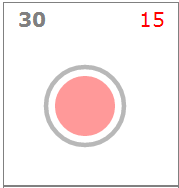
\includegraphics[scale=.25]{images/goldilocks-circle-small.PNG}
& 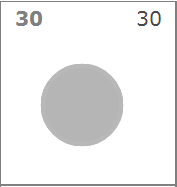
\includegraphics[scale=.25]{images/goldilocks-circle-justright.PNG}
& 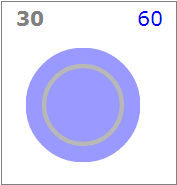
\includegraphics[scale=.25]{images/goldilocks-circle-large.PNG}\\ \\

$\mathbb{E}_{\empirical{}}\left[\vec{f}\right] 
- \mathbb{E}_{{p_{\vec{\theta}}}}\left[\vec{f}\right]$
%, and $\nabla_{\vec{\theta}} F$
& {\bf \color{red} \texttransparent{.55}{ red } }
& {\bf \color{gray}\texttransparent{.6}{ gray } }
& {\bf \color{blue} \texttransparent{.6}{ blue } }\\  \\
\vspace{.5em}

$\nabla_{\vec{\theta}} F$ 
& 
\includegraphics[scale=.25]{images/goldilocks-gradient-small.PNG}
& 
\includegraphics[scale=.25]{images/goldilocks-gradient-justright.PNG}
& 
\includegraphics[scale=.25]{images/goldilocks-gradient-large.PNG}\\ \\ 

\end{tabular}
\caption{Color and area indicate differences betwen the empirical
  distribution (gray outline) and model distribution. Red (or blue)
  indicates a model probability or parameter that should be
  increased (or decreased) to fit the data.}
\label{fig:colorsize_inventory}
\end{figure}

Winning either game with more complex models becomes instructively
difficult and tedious. 
The student may use \textit{hints}, such as
viewing components of the gradient (Figure~\ref{fig:gradients}), or 
clicking a button to havethe system follow the gradient.  

A main tenet of this manipulative is the benefit of ``learning-by-playing.'' 
Once comfortable with the provided model and data, the student can begin to play 
around with the dataset and model options. These utilities, such as
generating a new random challenge and experimenting with regularization, 
are described more in Section \ref{sec:lessons}.

The particular game being played in a lesson is described in the
instruction area. The instructions explain what the data and task are, justify modeling
choices, introduce new functionality and ask lesson-specific questions. For more technical 
explanations and derivations, or for additional practice questions, 
they may direct the student to auxiliary material provided with the code; it is designed to explain 
the physical intuitions gained and act as a self-check on one's understanding. 

The instructions and auxiliary material can help a student explore, but sometimes the 
student may just need to roam freely. To encourage this, the student can utilize any number of 
\textit{tooltips}, or hints/information that appear when a student hovers the cursor over an item. 
Tooltips are important because they provide guidance about whatever the student is thinking about \textit{right then}.
Many of them that come preloaded transcend individual lessons: some are static (e.g., what is the 
log-likelihood bar showing), while others 
dynamically update with changes to the model (e.g., the tooltips on the feature sliders show the 
observed and expected counts for that feature).  
This means students see the tooltips repeatedly, which can help them absorb and reinforce concepts over an extended 
period of time. Mutually referring tooltips (e.g., the log-likelihood score, regularization, and the 
gradient) both solidify growing intuition and encourage constructive play. Students who like to learn by
browsing and experimenting can point to various tooltips and get a sense of how the different 
concepts fit together. This allows those so inclined to go beyond the current lesson and make conceptual 
connections.

\subsection{The Instructor Interface: Creating and Tailoring Lessons}\label{sec:tailoring}

To support a wide-range of lessons, the manipulative has support for twelve predefined shape and fill combinations.
As seen in Figure \ref{fig:shape_inventory}, the available shapes are circles, triangles, squares and pentagons,
where each can be solid, striped or hollow.

The instructor must be able to tailor lessons to his or her students' needs, 
interests, and abilities. For instance, it may be appropriate to reason about different types of shapes
when introducing students to log-linear models, but eventually NLP students will want to think about 
NLP problems, whereas vision students will want to think about vision problems: we have designed the manipulative to handle text
and arbitrary images as well.

\begin{figure}[t]
\begin{center}
\centering
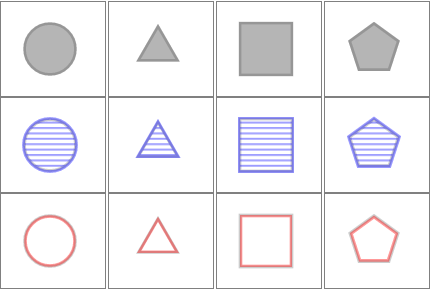
\includegraphics[scale=.5]{images/different_shapes_fills3x4.PNG}
\caption{Inventory of available shapes and fills. Normally color is indicative of 
the sign of \eqref{eqn:obsexp}, but here they are solely provided as example. 
Text and images (not shown) may also be included.}
\label{fig:shape_inventory}
\label{fig:inventory}
\end{center}
\end{figure}

Tailoring lessons to the students' needs is as simple as editing a couple text files. These must detail:
\begin{inparaenum}[(1)]
\item a set of features, 
\item a set of contexts, and
\item for each context, a set of uniquely featurized events, including counts and visual positions.
\end{inparaenum}
These simple requirements allow one to describe some rather involved models. For example, some of 
the features may be marked as ``hidden'' to the student, thereby allowing the student to experience 
model mismatch. If the set of contexts is missing, the model is assumed to contain only 
one context and be globally normalized. Note that the visual positioning information is pedagogically 
important: aligning objects by orthogonal descriptions, e.g., circles vs. triangles or solid vs. striped, 
can make feature contrasts stand out more.

The configuration files can turn off certain features on a per-lesson basis (without programming).  This is 
useful for, e.g., hiding the ``solve'' button in early lessons, adding new tooltips or adapting existing 
ones to emphasize different concepts in different lessons.\footnote{It is theoretically possible to provide arbitrarily targeted 
feedback, such as hints that depend on $\vec{\theta}$ and observed data counts. Code included in a particular lesson's instructions 
may suffice for one-off explanations but a more general solution should consider extending the back-end 
(Section \ref{sec:backend}). As our focus was on developing a general, wide-reaching tool, and such state-dependent 
hints would have impeded our goal, the manipulative currently has neither functionality. Under its open-source terms, 
instructors are free to extend it.}

\subsection{Back-End Implementation}\label{sec:backend}
The virtual manipulative is designed to be widely available and have no start-up cost. 
Aside from reading the data, model and instructions from the web server, it is fully 
client-side. The Javascript back-end uses common and well-supported open-source 
libraries for cross-browser compatibility and visualization.\footnote{Specifically and in order, 
\texttt{d3} (\url{d3js.org/}),
\texttt{jQuery} (\url{jquery.com/}), 
\texttt{jQuery UI} (\url{jqueryui.com}),
\texttt{jQuery Tools} (\url{jquerytools.org/}), and
\texttt{qTip} (\url{craigsworks.com/projects/qtip/}).}
The manipulative relies on certain capabilities from the HTML5
standard; unfortunately, not all current browsers support these
capabilities.
%\NoteJE{which browsers don't?}  
%\NoteFF{Internet Explorer; annoyingly, IE $< 10$ doesn't work though
%most users who use IE fall into that category.}
The tool works with recent versions of Firefox, Chrome and Safari and 
our students did not have trouble running it on them.
%\NoteJE{true?}
%\NoteFF{I don't have numbers to back it up, but generally I'd say yes.
%A couple people had issues with earlier versions of Firefox, but that was FF $< 11$. 
%Once I told them to upgrade it worked.
%
%More strongly, I can say that I've tested it in recent versions of the above
%three browsers. Some work better than others (e.g., Chrome is ``smoother'' 
%than FF), but nothing is broken.}

% so we do not believe this restriction to be unreasonable, 
% especially as all browers adopt widely used standards.

%The manipulative attempts to be responsive to an individual user's browser and display options, and 
%heuristically make efficient use of available space. That being said, higher resolution/larger displays 
%are desirable when dealing with the full model and some of the larger datasets introduced in later 
%lessons (see Section \ref{sec:conditionallessons}).
%
%mention that some ui considerations can result in very slight rounding errors
%
%solver: gradient ascent is simple (except for $\ell_1$ regularization), but it can take some finessing to make it visually appealing. We recursively call the solve function on a polynomial-decreasing schedule
%
%sigmoidal scaling for sliders, log-likelihood bars

%%%%%%%%%%%%%%%%%%%%%%%%%%%%%%%%%%%
%%%%%%%%%%%%%%%%%%%%%%%%%%%%%%%%%%%
%%%%%%%%%%%%%%%%%%%%%%%%%%%%%%%%%%%

\section{Pedagogical Aims}\label{sec:aims}

\subsection{Feature Design and Modeling Considerations}

Given a dataset $\Data{}$ of $N$ $(x, y)$ pairs, one of the initial decisions 
to make is \textbf{choosing an appropriate model} and distribution family. 
As argued above, for this manipulative we focus on contrasting exponential families 
\eqref{eqn:loglin} with what students may initially posit, the empirical 
distribution \eqref{eqn:empirical_distr}. While pragmatically the most important 
consequence of this modeling decision is that of proper feature design, one should 
understand certain underlying statistical properties of the model: what estimators 
exist and how ``good'' are they? How does \eqref{eqn:loglin} generalize other 
distributions: $\vec{\theta} = 0$ yields the uniform distribution, but can you match 
the empirical? What constraints does the model satisfy and what practical implications
are there?
%How does this relate to the maximum entropy view?
% (if any; eg., maxent formulation or empirical
%MLE?)
 
We contrast conditional models and globally normalized ones
$p_{\vec{\theta}}\left(y\right)$. Although
these context-unaware models allow students to focus on
understanding some of the core underlying mathematical concepts of
exponential models, such as feature interations and weight tradeoffs,
there are important differences between global and conditional models
that must be understood. For instance, conditional models can share 
features across conditions, helping generalize to unseen context-outcome 
pairs and maximizing the regularized objective.

The modeler has the onus of proper \textbf{feature design}. Broadly, what discriminative features 
help to model underlying data attributes? There are a number of at-times complex interactions 
to consider. Say we define a globally 
normalized model over solid circles, striped circles, solid triangles and striped triangles. 
The first features we might consider are contrasting indicator functions for whether a shape
is a circle or is solid, as in Figure \ref{fig:lesson1}. Which of the two games can the student 
``win'' using this two feature model and how might the empirical distribution affect the result? 
Will more features always help? Why might partitioning binary 
features be redundant in some cases (definining both circle and triangle features for the above example), 
yet insufficient in others?
%\footnote{Those with knowledge of statistics might benefit 
%from a discussion of the importance of rank in exponential families.}

The empirical distribution is concerned with \textit{type} counts, but log-linear models 
deal with descriptions of types; thus we can instead talk about \textbf{feature counts}. Our 
manipulative allows exploration of these two different counts and how they affect the 
feature weights. For example, if a feature is predicted to occur less often than it actually does, 
we should raise its weight. But raising that weight 
may affect the quality of all the other weights, so fitting one weight in
isolation may reduce or reverse the need to raise other weights. How can you mitigate  
adverse effects and get to the solution quickly, even in complex models?

Generally, both the number and range of features affect the expressive 
power of the model, as with enough features you can fit any distribution. But this expressiveness 
has a cost, as too many features can lead to overfitting. 
In one particularly important case, a feature for each $(x,y)$ pair allows an unregularized model to fit the 
data perfectly. 
Similarly, defining features that everything (or nothing) has can make the weights 
take extreme values (go to $\pm \infty$). Further, though features are commonly binary, 
this is not a strict requirement: defining non-binary feature functions, such as one that fires in 
proportion to some property of the datum (e.g., the number of sides of a shape) can affect the
proportions of feature counts. How does this interact with the amount of training data?

Our manipulative must generalize the above points to conditional models. Students should 
understand the effect the amount of data (per context) has on what features are appropriate to define. 
In particular, how do the marginal counts affect the resulting distributions, feature 
weights and the results of the matching and log-likelihood games? 
While exploring what backoff features are, and how and why they are useful, is important in its own right, 
it is important to connect them to smoothing, a topic with which some students may have previous experience. 
Understanding which features influence 
what conditional distributions, e.g., that features defined on conditions have no effect on conditional distributions, 
helps unite previously introduced concepts such as feature definition and model expressiveness considerations.

% defined over \Data{} , we are interested in estimating distributions 
%\begin{equation}
%p_{\vec{\theta}}\left(y\ \mid\ x\right) = \frac{u(x, y)}{\sum_{y'} u(x,y')},
%\label{eqn:conditional_loglin}
%\end{equation}
%from the unnormalized scores $u(x,y)$
%\begin{eqnarray}
%u(x,y) & = & \exp{\left(\vec{\theta}\cdot \vec{f}(x,y)\right)}.%\\
%%& = & \exp{\left(\sum_{k=1}^K \theta_k f_k(x,y)\right)}.
%\end{eqnarray}

%Therefore, we also 

\subsection{Importance of the Objective and Parameter Estimation} % and Evaluating the Model}

We summarize the model's quality via the regularized conditional
log-likelihood \eqref{eqn:reg_ll}.  
The maximizer is the $\vec{\theta^*}$ that solves equation \eqref{eqn:grad}:
\begin{equation}
\begin{aligned}
%\begin{split}
\nabla_{\vec{\theta}} F
 = &
\ \mathbb{E}_{\empirical{}}\left[\vec{f}(X,Y)\right] 
- \mathbb{E}_{{p_{\vec{\theta}}}}\left[\vec{f}(X,Y)\right]\\
 & - C \nabla_{\vec{\theta}}R(\vec{\theta})
\label{eqn:grad} \\
%= &\ \mathcal{C}(\empirical{}, p_{\vec{\theta}}) - C \nabla_{\vec{\theta}} R(\vec{\theta})\\
 = &\ 0.
%\end{split}
\end{aligned}
\end{equation}
Many important concepts are encapsulated in \eqref{eqn:reg_ll} and \eqref{eqn:grad}. 
Some are new while others provide an alternative view
on concepts already introduced. We highlight these connections when possible.

We believe the most important concept is that the gradient of (unregularized)
maximum likelihood is the \textbf{difference 
between observed and expected feature counts}:
\begin{equation}
\ \mathbb{E}_{\empirical{}}\left[\vec{f}(X,Y)\right] 
- \mathbb{E}_{p_{\vec{\theta}}}\left[\vec{f}(X,Y)\right].
\label{eqn:obsexp} 
\end{equation}
Students have already been introduced to this when considering the difference between type and 
feature counts, and how expectation proportions affect how much one needs to change a given feature weight: 
now, with the gradient, they can better understand why, and thus justify and strengthen their developing intuitions. 

For students with limited-to-no prior numerical optimization experience, the next 
important idea is what it means to ``follow'' the gradient up the convex ``hill,'' and that doing so will 
\begin{inparaenum}[i)]
\item actually yield a solution, even though a closed-form solution is not generally available, and
\item not decrease the objective.\footnote{We focus on gradient ascent but other parameter estimation methods 
exist, such as variants of iterative scaling, and first- and second-order gradient algorithms. The most popular 
methods have relied on quantities similar to \eqref{eqn:obsexp}, which, as shown in Figure \ref{fig:colorsize_inventory} 
and discussed above (\S\ref{sec:aims}), is 
one of the most important concepts we illustrate. See 
\newcite{berger-dellapietra-dellapietra-1996} and \newcite{malouf2002comparison}. }
\end{inparaenum}
The importance of the convexity of \eqref{eqn:reg_ll} generalizes these two observations.\footnote{Advanced 
students might try ``breaking'' convexity, e.g., what happens when $C < 0$?}
% $\vec{\theta^*}$ that solves \eqref{eqn:reg_ll}.
Students should understand that matching the empirical distribution will generally maximize the (unregularized) log-likelihood, 
though that overfitting is possible and may result in a larger log-likelihood than the true generating distribution yields.

We may use the gradient to further illustrate feature modeling considerations. The most obvious is to show how 
minimizing a single isolated $|\frac{\partial}{\partial \theta_k} F|$ might adversely affect another partial 
$\frac{\partial}{\partial \theta_{k'}}F$. Additional connections to differences in type and feature counts should be 
made: even if the model distribution does not fully match the empirical, expected and observed feature 
counts should match.

When we include regularization, we consider $R(\vec{\theta}) = \|\vec\theta\|_1$, and 
$R(\vec{\theta}) = \|\vec{\theta}\|_2^2$. This contrasts encouraging sparsity vs.  
heavily preferencing away from large feature weights.\footnote{Our optimizer special-cases 
the non-differentiable $\ell_1$ regularization, but we inform the students of this difficulty.} 
Related exploration involves how the penalty coefficient $C$ affects the overall solution and game outcomes.

Underlying the above concepts is \textbf{general machine learning} and 
\textbf{statistical knowledge}. These include what estimators are,  how different data or model configurations 
affect their quality, and how to limit adverse or prevent lower quality estimators. For example, 
a small sample size leads to estimators with higher variance; regularization is a way to mitigate that, albeit at the expense of 
the training log-likelihood. 
Similarly, why can regularization be considered a form of smoothing that fits the data 
imperfectly? The model might have fewer parameters than 
outcomes, or it might forgo many parameters to avoid being penalized by 
the regularizer.  Further, to limit regularization penalty, the model can make 
use of backoff features and not just fine-grained features, thereby resulting 
in \textit{backoff smoothing}. These concepts are connected to the expressiveness 
considerations introduced in feature modeling.

We should note that we are \textit{not} concerned with efficiency issues, e.g.,  
tractably computing the normalizers $Z(x)$. Efficiently computing the normalization 
factor is a crucial component to practical log-linear models, but our primary concern is to provide a virtual 
manipulative that imparts a near-physical intuitive understanding of log-linear models. See Section 
\ref{sec:history} or \newcite{smith-2011} for strategies on computing the partition function. 

%%%%%%%%%%%%%%%%%%%%%%%%%%%%%%%%%%%
%%%%%%%%%%%%%%%%%%%%%%%%%%%%%%%%%%%
%%%%%%%%%%%%%%%%%%%%%%%%%%%%%%%%%%%


\section{Provided Lessons}\label{sec:lessons}
Here we provide an overview of the \NumLessons{} available lessons. This is intended as a 
summary of the major concepts from the previous sections; we encourage the reader to 
walk through the tutorial to attempt the activities and read all the questions. We have tried to 
separate the lessons that build intuition from the ones focused on specific tasks or problems; this helps 
the student solidify the fundamentals and facilitates future development by providing what might be considered 
``core'' and ``auxiliary'' sets of lessons.

These core lessons start with \textbf{1}--\textbf{5}, which provide the basic introduction to log-linear modeling. We keep 
the models simple and incrementally build intution, and only consider joint models over shapes. The focus is 
on feature design. We start by comparing models over four shapes with two and four features. 
Next we hide certain generating features from the students: they 
consider what is going on in this model mismatch exercise, and a possible way to handle it. We play both the 
matching and log-likelihood games, comparing and contrasting them. Students also explore 
non-binary features and what it means for each game.\footnote{Students had difficulty with non-binary features; 
we have since improved the lessons to explore \eqref{eqn:obsexp} in greater depth.} 

Having begun to develop the appropriate intuition, lessons \textbf{6}--\textbf{8} introduce 
additional outcomes, and as a result, larger models. To deal with this complexity, we describe the convex 
objective and its gradient 
(Figure \ref{fig:gradients}), 
automatically solving for $\vec{\theta}$ via gradient ascent, and how a larger partial derivative means the objective is more 
sensitive to changing that feature. We connect the gradient, specifically computing observed and expected feature 
counts, with the previous lessons involving model mismatch; this allows students to better understand what the 
model was learning and why. 
Students can use the gradient hints and solver to watch $\vec{\theta}$ climb up the objective ``hill'' to the global maximum, 
partly illustrating the implications of a convex objective for our model's estimator.
%\footnote{There is with caveat of possibly stopping prematurely---``circling up'' the bowl.

\begin{figure}[t]
\centering
\small
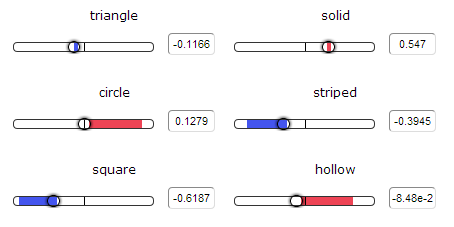
\includegraphics[scale=.65]{images/gradient-lesson7.PNG}
\caption{Gradient components use the same color coding as given in Figure \ref{fig:colorsize_inventory}. The length of each component indicates its potential effect on the objective, and not its magnitude.}
\label{fig:gradients}
\end{figure}

We also introduce additional manipulative functionality and encourage their use to 
explore log-linear models. For instance, students can generate secret oracle weights and 
fit a model to data sampled from those new weights. Students can also ``cheat'' and look at the true 
weights,  and question why estimates of $\vec{\theta}$ might be different from the true parameters 
(sampling error).

Having explored the gradient, lessons \textbf{8}--\textbf{10} consider more advanced topics in joint 
modeling. The first is regularization: how does regularization help with unseen data? Students are encouraged 
to play with the regularization coefficient, the amount of data and both $\ell_1$ and $\ell_2$ regularizers to 
explore the effects on model quality.

Lessons \textbf{11}--\textbf{13} introduce conditional models and convey some of the basic differences between 
conditional and globally normalized models. Students use a conditional model with shared features to model 
heavily skewed data, which illustrates how both the matching and log-likelihood games differ under conditional vs. 
joint models. We explain, via modeling syntactic parses, how shared conditional features can help more accurately 
model a context-specific outcome $\mathcal{Y}(x)$.

Lessons \textbf{14}--\textbf{15} further explore informed feature design in conditional models. 
Specifically in lesson \textbf{14}, we add a feature for each context and the students are asked what happens 
when we solve and why; that is, why context-only features do not move from their initial 0 values. 
In lesson \textbf{15}, we consider conjoined ``bigram'' features as a way to successfully incorporate 
contextual information into the model. We retain the original ``unigram'' (outcome) features, and explore
how the regularizer breaks parameter setting ties.

Lesson \textbf{16} begins the application-driven lessons. It extends the ``unigram'' and ``bigram'' concepts 
from the previous lesson to create a ``bigram language model.'' We step through the design of three general 
features that look at the event and the context together and ask open-ended questions that cause students 
to ponder estimation issues in conditional sequence models even when there is no model mismatch.
%Even though the data were generated from the ``true'' model, how well does the model fit the observed data sample, and how well can the model recover the ``true'' weights? Should regularization be used to answer these questions? What should you do if you need a very good estimate of those weights?

Finally, we apply log-linear modeling to the task of text categorization (spam detection). This lesson demonstrates to students how to encode logistic regression in our framework, and so 
we first ask some simpler questions to make sure they understand what is going on and what the conditional models actually mean.
Then, we can ask particular questions and make sure they understand how the feature modeling experience gained in 
prior lessons should be applied in practice. We also ask them to think about how to extend the approach to do three-way classification 
of a phrase (e.g., as \texttt{spam}, \texttt{work}, or \texttt{fun}).
%What kind of information below indicates that a particular training phrase has been labeled as spam?
%Which are the two test phrases included below? How do you know?
%If you train this model without regularization, what happens to the log-likelihood and the weights? Why?
%If you train this model with regularization, how does it classify the two test phrases? Look at the weights: what features helped it make this classification?
%You might think that 'fortune' fires on any phrase that contains the word 'fortune'. But lesson 14 suggests that can't quite work. Let's be precise: what (context,outcome) pairs is 'fortune' really defined to fire on?
%mentions money is a binary feature. What are some words that cause it to fire? How did you find out?
%Is the feature 'yada' a binary feature, or a counting feature? That is, does fyada return 1 or 3 on yada yada yada? How did you find out?
%Which of the non-spam messages does your trained model think is spammiest? How do you know?


%%%%%%%%%%%%%%%%%%%%%%%%%%%%%%%
%%%%%%%%%%%%%%%%%%%%%%%%%%%%%%% 

\section{Select Applications and Extensions} \label{sec:history}
We designed the tool to be extended and adapted to various needs. 
The following summary of log-linear applications serves to inspire 
further improvements in log-linear modeling education.

Conditional log-linear models were first popularized in computational
linguistics by a group of researchers associated with the IBM speech
and language group, who called them ``maximum entropy models,'' after
a principle that can be used to motivate their form
\cite{jaynes-1957}.  They applied the method to various binary or
multiclass classification problems in NLP, such as prepositional
phrase attachment \cite{ratnaparkhi-1994}, text categorization
\cite{nigam-lafferty-mccallum-1999}, and boundary prediction
\cite{beeferman-berger-lafferty-1999}.

Of particular importance for NLP, these models can be also used for
structured prediction problems such as tagging, parsing, chunking,
segmentation, and language modeling.  A simple strategy is to reduce
structured prediction to a sequence of multiclass log-linear
predictions \cite{ratnaparkhi-1998}.  A more global approach---used in
the original ``maximum entropy'' papers---is to use \eqref{eqn:loglin}
to define the conditional probabilities of the steps in a generative
process that gradually produces the structure
\cite{rosenfeld-1994,berger-dellapietra-dellapietra-1996}.  This idea
remains popular today and can be used to embed rich distributions
into a variety of generative models \cite{bergkirkpatrick-et-al-2010}.
For example, a PCFG that uses richly annotated nonterminals involves a
large number of context-free rules.  Rather than estimating their
probabilities separately, or with traditional backoff smoothing, a
simpler approach is to use \eqref{eqn:loglin} to model the probability
of all rules given their left-hand sides, based on features that
consider subsets of the nonterminal annotations.\footnote{E.g., case,
  number, gender, tense, aspect, mood, lexical head.  In the case of a
  terminal rule, the spelling or morphology of the terminal symbol can
  be considered.}  

A final approach to structured prediction is to
simply predict the structured output all at once, so that $y$ is a
large structured object. One can restrict ${\cal Y}(x)$ before training
\cite{johnson-et-al-1999}, or use techniques such as dynamic
programming or sampling, as in linear-chain conditional random fields
\cite{lafferty-mccallum-pereira-2001} and whole-sentence language
modeling \cite{rosenfeld-chen-zhu-2001}. 

\NoteJE{list
  other people's NLP homework assignments or practical exercises that
  use maxent.  I bet you could find a few good assignments on the web,
  including in the NLTK book.}
\NoteFF{NLTK: Select one of the classification tasks described in this chapter, such as name gender detection, document classification, part-of-speech tagging, or dialog act classification. Using the same training and test data, and the same feature extractor, build three classifiers for the task: a decision tree, a naive Bayes classifier, and a Maximum Entropy classifier. Compare the performance of the three classifiers on your selected task. How do you think that your results might be different if you used a different feature extractor?; Berkeley  maxent for proper noun classification, or POS tagging} \url{http://www.cs.berkeley.edu/~klein/cs288/}


%%%%%%%%%%%%%%%%%%%%%%%%%%%%%%%
%%%%%%%%%%%%%%%%%%%%%%%%%%%%%%%

\section{Conclusion}
We have introduced an open-source, web-based virtual manipulative for
log-linear models. Included with the code are
\NumLessons{} lessons, with possible assignment questions, and an auxiliary handout that 
gives a formal treatment of the necessary derivations.
A version is available at \WhereToFind{}.

%%%%%%%%%%%%%%%%%%%%%%%%%%%%%%%
%%%%%%%%%%%%%%%%%%%%%%%%%%%%%%% 

\paragraph*{Acknowledgements}
We would like to thank the anonymous reviewers for their helpful feedback and suggestions 
and the entire Fall 2012 Natural Language Processing course at 
Johns Hopkins.


\bibliographystyle{acl}
\bibliography{tnlp}

\end{document}
